\documentclass[11pt, a4paper, titlepage, openright]{article}

\usepackage{amsmath}
\usepackage[font=small,labelfont=bf]{caption}
\usepackage{float}
\restylefloat{figure}
\usepackage{graphicx}
\usepackage{hyperref}
\usepackage{mathtools}
\usepackage[titletoc, title]{appendix}
\usepackage{listings}
\usepackage{color}
\usepackage{fixltx2e}
\usepackage[bottom]{footmisc}

\definecolor{dkgreen}{rgb}{0,0.6,0}
\definecolor{gray}{rgb}{0.5,0.5,0.5}
\definecolor{mauve}{rgb}{0.58,0,0.82}

\lstset{frame=tb,
  language=C++,
  aboveskip=3mm,
  belowskip=3mm,
  showstringspaces=false,
  columns=flexible,
  basicstyle={\footnotesize\ttfamily},
  numbers=none,
  numberstyle=\tiny\color{gray},
  keywordstyle=\color{blue},
  commentstyle=\color{dkgreen},
  stringstyle=\color{mauve},
  breaklines=true,
  breakatwhitespace=true,
  tabsize=3,
  showstringspaces=false,
  keepspaces=true, 
  columns=flexible
}

\begin{document}
%%%%%%%%%%%%%%%%%%%%%%%%%%%%%%%%%%%%%%%%%
% University Assignment Title Page
% LaTeX Template
% Version 1.0 (27/12/12)
%
% This template has been downloaded from:
% http://www.LaTeXTemplates.com
%
% Original author:
% WikiBooks (http://en.wikibooks.org/wiki/LaTeX/Title_Creation)
%
% License:
% CC BY-NC-SA 3.0 (http://creativecommons.org/licenses/by-nc-sa/3.0/)
%
% Instructions for using this template:
% This title page is capable of being compiled as is. This is not useful for
% including it in another document. To do this, you have two options:
%
% 1) Copy/paste everything between \begin{document} and \end{document}
% starting at \begin{titlepage} and paste this into another LaTeX file where you
% want your title page.
% OR
% 2) Remove everything outside the \begin{titlepage} and \end{titlepage} and
% move this file to the same directory as the LaTeX file you wish to add it to.
% Then add \input{./title_page_1.tex} to your LaTeX file where you want your
% title page.
%
%%%%%%%%%%%%%%%%%%%%%%%%%%%%%%%%%%%%%%%%%

%----------------------------------------------------------------------------------------
%	PACKAGES AND OTHER DOCUMENT CONFIGURATIONS
%----------------------------------------------------------------------------------------
\begin{titlepage}

\newcommand{\HRule}{\rule{\linewidth}{0.5mm}} % Defines a new command for the horizontal lines, change thickness here

\center % Center everything on the page

%----------------------------------------------------------------------------------------
%	HEADING SECTIONS
%----------------------------------------------------------------------------------------

\textsc{\LARGE University of Antwerp}\\[1.5cm] % Name of your university/college
\textsc{\Large }\\[4cm] % Major heading such as course name
\textsc{\Large Scientific Programming}\\[0.5cm] % Minor heading such as course title

%----------------------------------------------------------------------------------------
%	TITLE SECTION
%----------------------------------------------------------------------------------------

\HRule
{ \huge \bfseries Second Session \\ \Large{Exercise 2}}\\ % Title of your document
\HRule \\[1.5cm]

%----------------------------------------------------------------------------------------
%	AUTHOR SECTION
%----------------------------------------------------------------------------------------

\begin{minipage}{0.4\textwidth}
\begin{flushleft} \large
Armin Halilovic - s0122210 % Your name
\end{flushleft}
\end{minipage}
~
\begin{minipage}{0.4\textwidth}
\begin{flushright} \large
\end{flushright}
\end{minipage}\\[4cm]

% If you don't want a supervisor, uncomment the two lines below and remove the section above
%\Large \emph{Author:}\\
%John \textsc{Smith}\\[3cm] % Your name

%----------------------------------------------------------------------------------------
%	DATE SECTION
%----------------------------------------------------------------------------------------

\vfill % Fill the rest of the page with whitespace
{\large August 22, 2016}\\[3cm] % Date, change the \today to a set date if you want to be precise

%----------------------------------------------------------------------------------------
%	LOGO SECTION
%----------------------------------------------------------------------------------------

%\includegraphics{Logo}\\[1cm] % Include a department/university logo - this will require the graphicx package

%----------------------------------------------------------------------------------------


\end{titlepage}
\tableofcontents
\newpage

\section{Problem}
    We are given the following set of inequalities:
        \[ \begin{cases}
            1 \leq x \leq 3 \\
            -1 \leq y \leq 4 \\
            x^3 + y^3 \leq 29 \\
            y \geq e^x - 2
        \end{cases} \]

    These inequalities describe an irregular 2D figure. We will find the area of this figure using the Monte Carlo method to estimate areas and volumes, which in general looks like:
    \[ \int_{A}^{}f \approx (measure\ of\ A) * (average\ of\ f\ over\ n\ random\ points\ in\ A) \]

    \bigskip
    This will be done using C++ and the \href{http://www.gnu.org/software/gsl/}{GNU Scientific Library}. 
    In section~\ref{sec:solutions}, we will describe how we reached each solution, using the most important parts of the code.

\bigskip
\bigskip
\section{Using the program}
    All of the C++ code for the program can be found in the file main.cpp and in appendix A of this document.

    To compile and run the program, execute the following commands in the build/ directory:
\begin{lstlisting}
cmake ..
make
./numerical_integration.bin
\end{lstlisting}
    Do not forget the .bin extension.
    Output can be found in the console output of the program and in appendix B.1.
    
\newpage
\section{Solutions}
\label{sec:solutions}
    \subsection{Find the figure}
        From the given set of inequations, we can deduce that the figure is bounded by the functions
        \( \sqrt[3]{29 - x^3} \), \( e^x -2 \), and by the rectangle defined by the points \( (1, -1), (3, -1), (3, 4), (1, 4) \).
        The functions and rectangle are plotted in figure~\ref{fig:rect}. The marked area is the figure we want to know the area of.

        \begin{figure}[H]
            \begin{minipage}[b]{0.49\textwidth}
                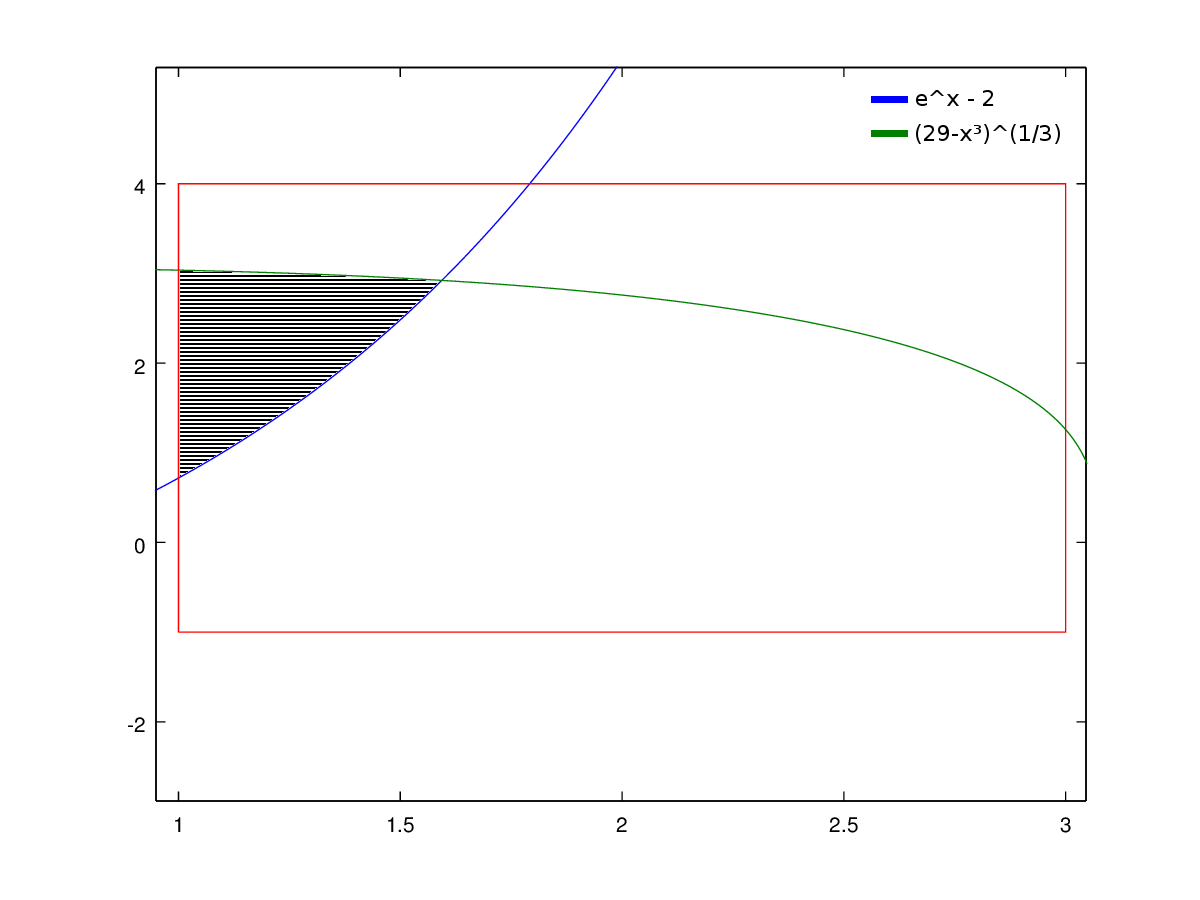
\includegraphics[width=12cm]{../images/rectangle}
            \end{minipage}
            \caption{The functions and rectangle defined by the given inequalities}
	        \label{fig:rect}
        \end{figure}
    
    \subsection{Choose a decent random number generator}
        We chose to use ranlxs0 as the random number generator for these solutions. ranlxs0 is based on the RANLUX algorithm. Generators based on the RANLUX
        algorithm offer the best mathematically-proven quality of randomness. Besides this, ranlxs0 is got a pretty high spot on GSL's preformance table\footnote{https://www.gnu.org/software/gsl/manual/html\_node/Random-Number-Generator-Performance.html}.
        These facts made ranlxs0 seem like a good choice. \\
        We use GSL's random number generation library as follows:
        
\noindent
\begin{minipage}{\linewidth}
\begin{lstlisting}
//Use c++11's random_device to create a random unsigned int to use as seed for the generator
std::random_device rd;
//Initialize the ranlxs0 random number generator
gsl_rng *r = gsl_rng_alloc(gsl_rng_ranlxs0);
//Seed the generator with a random number
gsl_rng_set(r, rd());

//Get a random number in [0, 1]
double randomNumber = gsl_rng_uniform(r);
\end{lstlisting}
\end{minipage}
    
    \subsection{Calculate the area}
        We are now ready to use the Monte Carlo estimation method. The red rectangle in figure~\ref{fig:rect} is the A in:
        \[ \int_{A}^{}f \approx (measure\ of\ A) * (average\ of\ f\ over\ n\ random\ points\ in\ A) \]
        How the algorithm is used is explained with the following code excerpt.

\noindent
\begin{minipage}{\linewidth}
\begin{lstlisting}[numbers=left]
double calculateArea(int n) {
    ...
    for (int i = 0; i < n; i++) {
        //gsl_rng_uniform(r) uniformly gets a random number in [0, 1]
        x = 2 * gsl_rng_uniform (r) + 1;
        y = 5 * gsl_rng_uniform (r) - 1;

        if ((gsl_pow_int(x, 3) + gsl_pow_int(y, 3) <= 29) and (y >= exp(x) - 2)) result++;
    }
    result /= n;
    result *= 2.0 * 5.0;
    ...
    return result;
}
\end{lstlisting}
\end{minipage}
        Lines 3 to 10 do the \( (average\ of\ f\ over\ n\ random\ points\ in\ A) \) part of the equation. Points (x, y) are chosen to lie within the given bounds
        of the rectangle. If they then lie in the marked part of figure~\ref{fig:rect}, a counter is incremented.
        Then, at line 10, the counter is divided by the total amount of points generated. \\
        The result of this then has to be multiplied by \((measure\ of\ A)\), which is simply the area of the rectangle. \\
        That's all, we can now calculate approximations of the area of the given figure using the function calculateArea, which takes as argument the amount of random points to generate.
    \subsection{Results}
        By calculating the area manually by integration, we found that the area of the figure is approximately 0.758. \\
        While experimenting with calculateArea with various values for n, we noticed that there is a high variance in the results we get. \\
        For example, when generating 1000 points, the resulting area can be somewhere between 0.65 and 0.85. \\
        
        \subsubsection{More points}
        \label{sec:morep}
            One way to improve the results is to simply generate (many) more points. Filling the figure with as many points as possible will lead to a better
            result, at the cost of more processing power. \\
            In the function calculateUntil(double e), an area is calculated for an \(n_0\), where \(n_0\) is randomly chosen to lie in [2000, 5000]. Then, 
            an area is calculated for \(n_{i+1} = 2n_i\) and compared to the previous result. This is repeated until the difference between two 
            sequential results is smaller than e. \\
            Then, in calcAvgOfN(int n, double e), this is done n times, and an average of the n calculations is returned. \\
            This solution improved the results, but is is not really a practical solution. \\
            To give an example, calcAvgOfN(10, 0.01) narrowed the resulting area down to range from around 0.745 to 0.765 
        \subsubsection{Smaller rectangle}
            A better way to improve the results is to use a rectangle that wraps the figure tighter. The rectangle we used previously left a lot of open 
            space around the figure. Because of this, we need many more points to get a result that we could get with a smaller rectangle. \\
            To construct the smaller rectangle:
            \begin{itemize}
                \item The left x value, \(x_0\), stays the same.
                \item The right x value, \(x_1\), is the cross point of \( \sqrt[3]{29 - x^3} \) and \( e^x -2 \)
                \item The bottom y value is the minimum of \( \sqrt[3]{29 - x^3} \) and \( e^x -2 \) on the interval \([x_0, x_1]\)
                \item The top y value is the maximum of \( \sqrt[3]{29 - x^3} \) and \( e^x -2 \) on the interval \([x_0, x_1]\)
            \end{itemize}
            For these values, we find 1, 1.59374, 0.718282 and 3.03659, respectively. 
            \newpage
            In figure~\ref{fig:rect2}, this new rectangle is depicted.
            We can clearly see that the ratio \(\frac{area\ figure}{area\ rectangle}\) is larger than the one with the previous rectangle. The result of
            this is that the same results as before can be achieved with fewer points generated.  \\
            This can be confirmed by using the function \begin{mbox}calcAvgOfN(10, 0.01, true)\end{mbox}\footnote{In the code, the boolean smallerRectangle will make the calculcations use
            the smaller rectangle instead of the given one.}. The output of this function can be seen appendix in~\ref{sec:consoleOut}. We can confirm that 
            when using the smaller rectangle, fewer points are generated to achieve approximately the same result.
            
            \begin{figure}[H]
                \begin{minipage}[b]{0.49\textwidth}
                    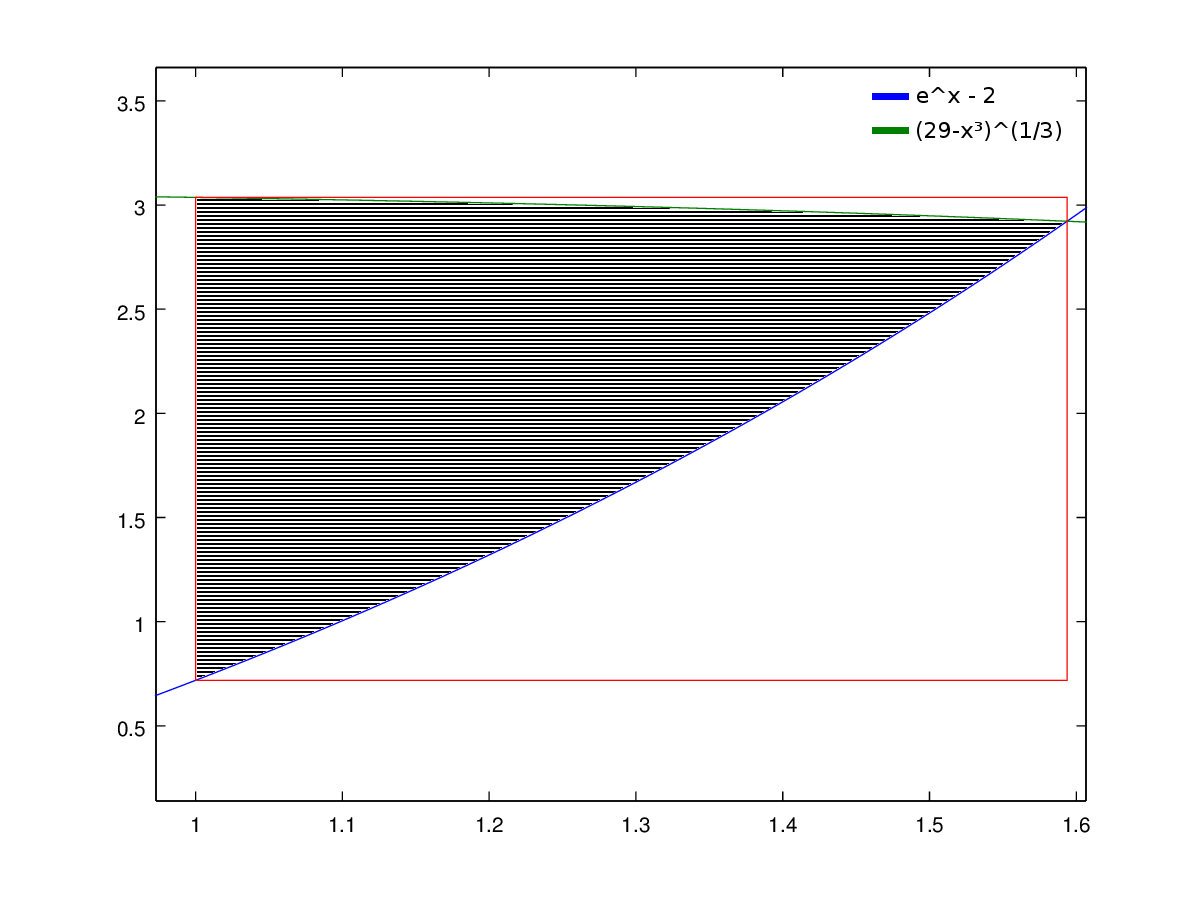
\includegraphics[width=12cm]{../images/rectangleSmaller}
                \end{minipage}
                \hfill
                \caption{The given functions and the smaller rectangle}
	            \label{fig:rect2}
            \end{figure}

\onecolumn
\appendix
\appendixpage
\addappheadtotoc

\section{Code}
	\subsection{main.cpp}
		\lstinputlisting[basicstyle=\scriptsize]{../main.cpp}
	\bigskip

\newpage
\section{Output}
\label{sec:output}
	\subsection{Console output}
	\label{sec:consoleOut}
		\lstinputlisting[basicstyle=\scriptsize, language=bash]{../consoleSampleOutput.txt}
    
\end{document}